\documentclass[aps,prb,reprint,showpacs,floatfix,superscriptaddress, onecolumn, nofootinbib, 9pt]{revtex4-2}

\usepackage{amsmath,amsthm,amssymb}
\usepackage{graphicx}% Include figure files
\usepackage{dcolumn}% Align table columns on decimal point
\usepackage{bm}% bold math
\usepackage{color}
\usepackage{epsfig}
\usepackage{multirow}
\usepackage{mathrsfs}
\usepackage{hyperref}
\usepackage{cleveref}
\usepackage{epstopdf}
\usepackage{subfigure}
\usepackage{autobreak}

\usepackage{physics}
\usepackage{bbm}

%Macros for mathematical notations

\newcommand{\V}[1]{\boldsymbol{#1}} %# vector
\newcommand{\M}[1]{\boldsymbol{#1}} %# matrix
\newcommand{\Set}[1]{\mathbb{#1}} %# set
\newcommand{\D}[1]{\Delta#1} %# \D{t} for time step size
\renewcommand{\d}[1]{\delta#1} %# \d{t} for small increment
\newcommand{\av}[1]{\left\langle #1\right\rangle } %take average

\newcommand{\sM}[1]{\M{\mathcal{#1}}} %matrix in mathcal font
\newcommand{\dprime}{\prime\prime} % double prime
%\global\long\def\i{\iota}
%\renewcommand{\i}{\iota} %i for imaginary unit
%\renewcommand{\i}{\mathsf i} %i for imaginary unit
\newcommand{\follows}{\quad\Rightarrow\quad} %=>
\newcommand{\eqd}{\overset{d}{=}} %=^d
\newcommand{\spe}[1]{\mathscr{#1}}  %important quantities in mathscr font
\newcommand{\eps}{\epsilon}

\newcommand{\ar}[1]{{\color{blue}#1}} % for authors' response


\begin{document}
\preprint{Preprint}

\title{First Response to Referee Comments for Manuscript BJ14850}
\author{Analabha Roy}
\date{\today}

\maketitle

\vspace{1em}

\noindent \textbf{Response to First Referee}

\begin{enumerate}
\item The referee says, ``\textit{The paper is littered with typographical errors and poorly worded sentences, which make it hard to read and understand.}"\\

\ar{
We sincerely regret this oversight and thank the referee for stressing the importance of properly correcting any errors and improving sentence structure. We have completed this task to the best of our abilities. In addition, we improved several of our figures and restructured sections of the material to improve clarity.
}
\item The referee says, ``\textit{The mathematical
expansion used made in going from Eq 6 to Eq 7, which seems central, makes utterly no sense in the supposedly high-frequency limit expansion being used. You'd need 4 h/omega to be small to truncate the Jacobi-Anger sum. But you need 4h/omega to be O(1) to lie at a root of J$_0$. So the approximation made is inconsistent with the regime in which the expression 7 is being used.}".\\

\ar{
We appreciate the referee bringing this up. We believe the question occurred as a result of a lack of clarity in our derivation. As a result, we have corrected and revised the writing in ``Section II. Interacting Dynamical Localization" as well as ``Appendix A," and clarified how we obtain the optimal values of the drive parameters amplitude $h$ and frequency $\omega$ that lead to localization during the $T_2-$cycle. For further clarity, we present an extended explanation below.\\

The moving frame Hamiltonian is defined in Eq.(6) in the manuscript as
\begin{equation}
    \hat{H}^{mov}(t) = \hbar\sum_{ij} J_{ij} \Big(\hat{\sigma}^y_i\hat{\sigma}^y_j\Big) e^{i 2\zeta(t)\hat{\sigma}^z_i}  e^{i 2\zeta(t) \hat{\sigma}^z_j},
    \label{eq:hmov}
\end{equation}
where $\zeta(t)\equiv \frac{h}{\omega}[1-\cos(\omega t)]$. Now, before we apply the Jacobi-Anger expansion to this expression, let us define $ A(\chi,\theta)\equiv\displaystyle e^{i\chi \cos(\theta)} = \sum_{n=-\infty}^{\infty} \mathcal{J}_n(\chi)e^{in\theta} $. In this case, $A$ is a function of two independent variables, $\chi$ and $\theta$, and $0\leq\theta\leq 2\pi$. The coarse-grained average $\bar{A}(\chi)$ is defined as the average of $A(\chi, \omega)$ across all values of $\theta$. Thus,
\begin{equation}
\bar{A}(\chi) \equiv \expval{e^{i\chi\cos(\theta)}}_{\theta} = \sum_{n=-\infty}^{\infty} \mathcal{J}_n(\chi) \expval{e^{in\theta}}_{\theta} =\mathcal{J}_0(\chi).
\end{equation}
In the paper, we also have two independent parameters, namely the driving frequency $\omega$ and amplitude $h$. These are connected to $\chi, \theta$ by a trivial linear map, $\chi=4h/\omega, \theta=\omega t$. Thus, we can obtain the coarse-grained average similarly to yield
\begin{equation}
    \bar{A}(h,\omega) \equiv \expval{e^{i\frac{4h}{\omega}\cos(\omega t)}}_t = \sum_n\mathcal{J}_n\left(\frac{4h}{\omega}\right)\expval{e^{i n \omega t}}_t = \mathcal{J}_0(\chi) ;  \forall{\chi}\in\mathbb{R},
    \label{eq:jacang}
\end{equation}
where our coarse-graining is over time scales $t\gtrsim 2\pi/\omega$, allowing us to average all harmonic oscillations to zero (regardless of the value of the amplitude), leaving behind only the constant $n=0$ term in the Fourier series on the RHS. The Rotating Wave Approximation (RWA) states that if $\omega \gg 1$, then  $\bar{A}(h,\omega)$ approximates $A(h, \omega t)$. The RWA does not impose any constraint on $h$.
This allows us to independently alter $\omega \gg 1$ \emph{and} $h \gg 1$ so that the ratio $\frac{4h}{\omega} \approx \order{1}$ without violating the RWA criteria. For example, if $\omega=100$ and $h\approx 60.1206\dots$, we get $\bar{A}(h,\omega)=\mathcal{J}_0(2.404\dots)=0$, and, because the RWA still holds due to the huge $\omega$, we may approximate $A(h,\omega t)$ by $0$.

Therefore, it is reasonable to approximate   $\hat{H}^{mov}$ in our manuscript by 
\begin{align}
	\hat{H}^{_{RWA}} = \hbar\sum_{ij} J_{ij} \Big(\hat{\sigma}^y_i\hat{\sigma}^y_j\Big) \mathcal{J}_0\Big(\frac{4h}{\omega}\Big)\Bigg[\mathbbm{1}\Bigg\{\mathcal{J}_0\Big(\frac{4h}{\omega}\Big) + \cos(\frac{4h}{\omega})\Bigg\} -\hat{\sigma}^z_i\hat{\sigma}^z_j \Bigg\{\mathcal{J}_0\Big(\frac{4h}{\omega}\Big) - \cos(\frac{4h}{\omega})\Bigg\} + \frac{i}{2} (\hat{\sigma}^z_i + \hat{\sigma}^z_j) \sin(\frac{4h}{\omega})\Bigg],
\end{align}
as long as $\omega\gg 1$ (say $\sim 10^2$). If we now adjust $h$ (also say $\gtrsim 10^2$) so that ($4h/\omega$) lies on a root of $\mathcal{J}_0(4h/\omega)$, then $\hat{H}^{_{RWA}}$ vanishes, resulting in full localization of the spin system during the $T_2$ cycles.

 We can strengthen our argument with numerical simulations of a simple driven TLS  where RWA is widely known to apply (and this phenomenon referred to as \textit{Coherent Destruction of Tunneling}~\cite{Grossmann1991, Ashhab2007}, or CDT) . Here, the Hamiltonian $\hat{\mathcal{H}}(t) = \hat{H}_0 + \hat{H}_1(t)$, and  
\begin{align}
\hat{H_0} &= \Delta \hat{\sigma}^x,\nonumber \\
\hat{H_1}(t) &= h \cos(\omega t)\hat{\sigma}^z.
\end{align}}
\begin{figure}[t!]
\begin{center}
	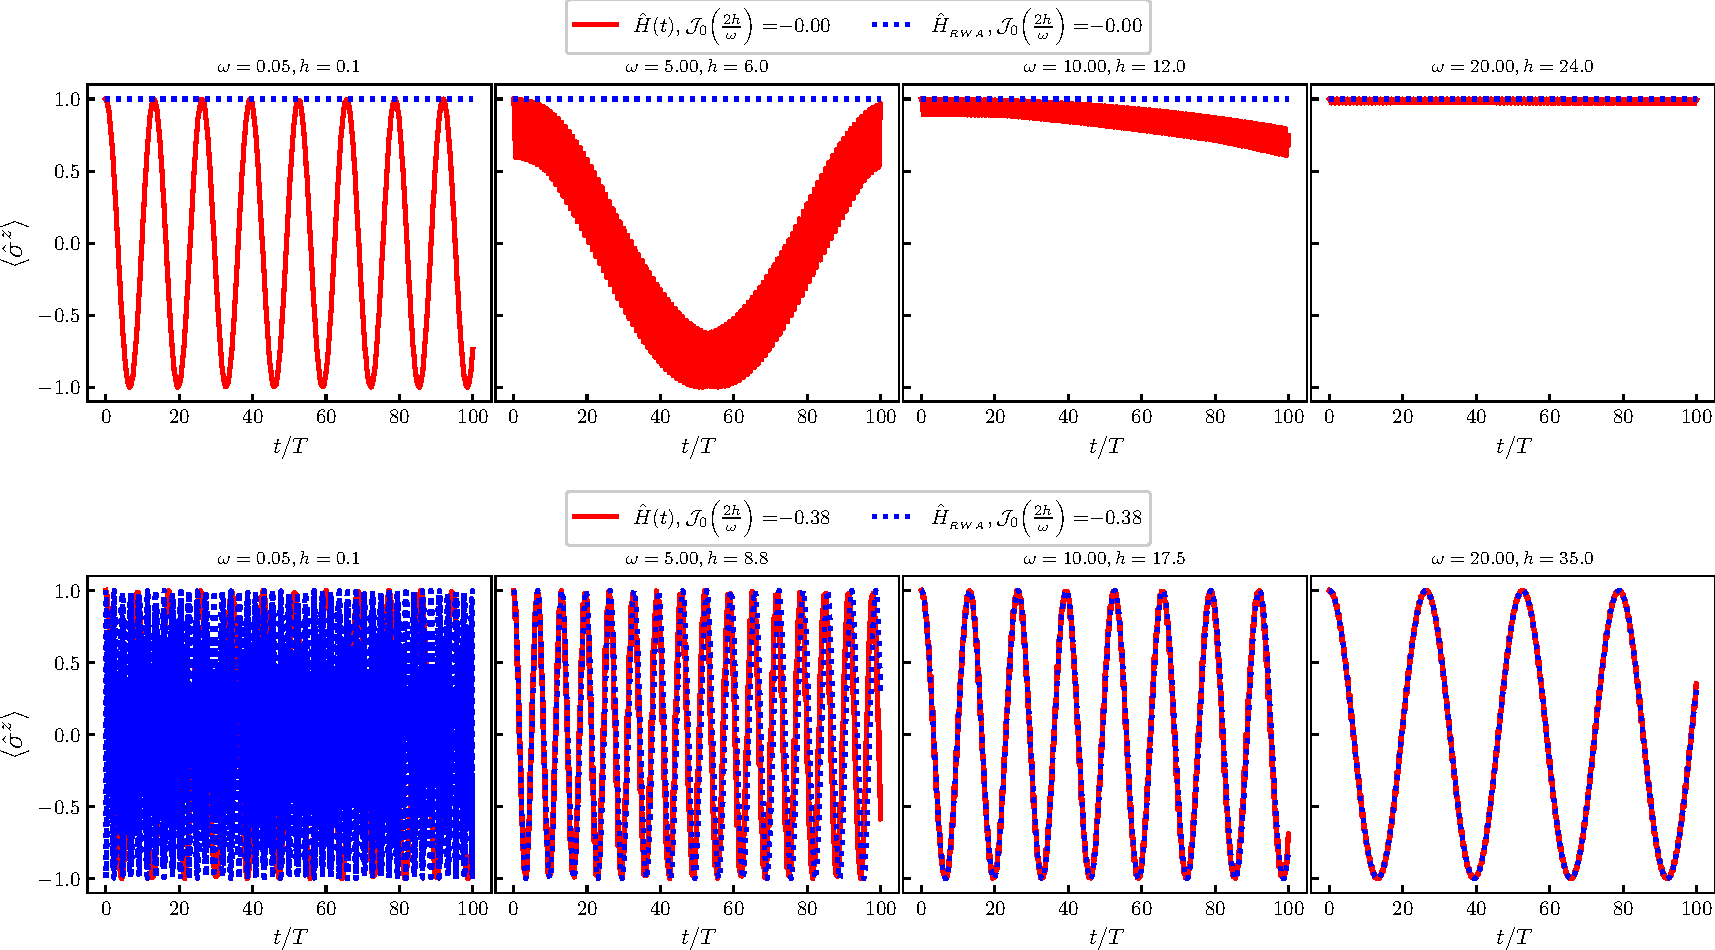
\includegraphics[height=9.5cm]{rwa_vs_exact_w_low_n_high_frz_nfrz.pdf}
\end{center}
\caption[] {Comparison of the exact time evolution and the RWA-approximated time evolution of the magnetization $\expval{\hat{\sigma}^z}(t)$ for the harmonically driven quantum two-level system (TLS). The evolution is performed from the eigenstate of $\sigma^z$ at $t=0$ for different drive frequencies $\omega$ with amplitudes $h$. The latter are set to values where $2h/\omega$ lies either at the first root of $\mathcal{J}_0\left(\frac{2h}{\omega}\right)$ (top panels), or a little away from it (bottom panels). The plots are presented in increasing order of $\omega$ from the left to right panels.}
\label{Fig:compare_exact_rwa}
\end{figure}
\ar{In the rotating frame obtained from the $\hat{H}_1-$propagator $\hat{U}(t) = \exp\big[-i \frac{h}{\omega} \sin(\omega t)\hat{\sigma}^z\big]$, the moving frame Hamiltonian is
\begin{align}
\tilde{\mathcal{H}}(t)^{mov} &=\hat{U}^\dagger(t) \mathcal{H}(t) \hat{U}(t) - i \hat{U}^\dagger(t) \partial_t \hat{U}(t)\nonumber\\
&= \hat{U}^\dagger(t) H_0 \hat{U}(t)\nonumber\\
&= e^{i \frac{h}{\omega} \sin(\omega t)\hat{\sigma}^z} \Big(\Delta \hat{\sigma}^x\Big) e^{-i \frac{h}{\omega} \sin(\omega t)\hat{\sigma}^z}
\end{align}
Now, let us define $\phi \equiv \frac{2h}{\omega} \sin(\omega t)$. Recalling $\hat{S}^{x,y,z} = \frac12 \hat{\sigma}^{x,y,z}$, we can expand the moving frame Hamiltonian as follows.
\begin{align}
\tilde{\mathcal{H}}(t)^{mov} &= e^{i \frac{2h}{\omega} \sin(\omega t)\hat{S}^z} \Big(2\Delta \hat{S}^x\Big) e^{-i \frac{2h}{\omega} \sin(\omega t)\hat{S}^z}\nonumber\\
&= 2\Delta \Big(\hat{S}^x \cos{\phi} - \hat{S}^y \sin{\phi}\Big)\nonumber\\
&= 2\Delta \bigg\{\hat{S}^x\cos\Big[\frac{2h}{\omega}\sin(\omega t)\Big] - \hat{S}^y\sin\Big[\frac{2h}{\omega}\sin(\omega t)\Big]\bigg\},
\end{align}
where we have used the Baker-Campbell Hausdorff formula, together with the angular momentum commutation relations $[\hat{S}^\mu, \hat{S}^\nu]=\epsilon_{\mu\nu\alpha}\hat{S}^\alpha$
Next, using the Jacobi Anger formula, we get
\begin{equation}
\tilde{\mathcal{H}}(t)^{mov} = \Delta \Bigg[\hat{\sigma}^x \bigg\{\mathcal{J}_0\Big(\frac{2h}{\omega}\Big) + 2 \sum_{n=1}^{\infty} \mathcal{J}_{2n-1}\Big(\frac{2h}{\omega}\Big)\cos(2n\omega t)\bigg\} -\hat{\sigma}^y\bigg\{2\sum_{n=1}^{\infty} \mathcal{J}_{2n-1}\Big(\frac{2h}{\omega}\Big) \sin\left[(2n-1)\omega t\right]\bigg\}\Bigg]
\label{eq:hexact}
\end{equation}
Now, applying RWA for $\omega \gg 1$ simply involves neglecting the fast-oscillating terms. This yields
\begin{equation}
\tilde{\mathcal{H}}(t)^{mov}\approx\hat{\mathcal{H}}^{_{RWA}} = \Delta \mathcal{J}_0 \Big(\frac{2h}{\omega}\Big) \hat{\sigma}^x,
\end{equation}
with the only constraint being that $\omega \gg 1$. As can be readily seen, the moving frame Hamiltonian almost vanishes when $\omega\gg 1, h\gg 1$, and $2h/\omega$ lies at a root of the zeroth Bessel function.

We have numerically evolved the exact Hamiltonian $\hat{\mathcal{H}}(t)$, as well as the RWA Hamiltonian $\hat{\mathcal{H}}^{_{RWA}}$, for multiple sets of drive parameters, both at and away from values where $2h/\omega$ lies on a root of $\mathcal{J}_0\left(\frac{2h}{\omega}\right)$. We have contrasted their dynamics by comparing $\expval{\hat{\sigma}^z}(t)$, obtained by using the QuTiP 'mesolve' integrator of the Schr\"odinger equation for both Hamiltonians. In both cases, the state of the system was set to the $+1$ eigenstate of $\sigma^z$ at $t=0$. The results are plotted in fig~\ref{Fig:compare_exact_rwa}. The top panels contain plots for the case where $(2h/\omega)$ lies on the first root of $\mathcal{J}_0$, whereas the bottom panels contain plots for when it does not. We have considered four different drive frequencies, ranging from small to high values ($\omega = 0.05, 5.0, 10.0, 20.0$) with appropriately adjusted drive amplitudes. The plots are arranged in order of increasing $\omega$ from the left to right panels of fig~\ref{Fig:compare_exact_rwa}. As can be readily seen, the exact and RWA results do not match very well when $\omega \lesssim 1$. However, as $\omega$ increases (together with $h$), they come closer, with slightly better matching away from the root than on it~\footnote{\ar{At the root, the expansion's zeroth mode disappears, allowing the $n=\pm 1$ mode to dominate. Its contribution is only visible at larger times, as seen in Fig~\ref{Fig:compare_exact_rwa} for $\omega=5, 10$, and can be lessened by hiking up $\omega, h$ to a point where it develops beyond experimentally accessible time scales.}}. For either cases, when $\omega=20 \gg 1$, the results match very well.

We hope that our response clarifies the methodology that we have used in our analysis.
}
\end{enumerate}

\noindent \textbf{Response to Second Referee}

\begin{enumerate}
\item The referee says,``The original work of Bruno on no-go-theorems for time crystals should be mentioned in the introduction: P. Bruno PRL 111, 070402(2013) "\\

\ar{
We thank the referee for the suggestion to mention Bruno's no-go theorem in the manuscript. We have introduced Bruno's work in the second paragraph of the introduction part.
}
\item The referee says,``The reference in 34 is incomplete "

\ar{    	
Thanks to the referee for alerting us to the problem with the reference to the Kuramoto \& Battogtokh article. We have tried to rectify it (please note that the reference has been repositioned due to additions), but were unable to find the original DOI to the peer-reviewed version. Thus, we retained the DOI to the arXiv version to prevent link-rot.}

\item The referee says, ``The time-evolution operator in Eq. 4 should contain a time-ordering operator "

\ar{
We thank the referee for detecting the mistake in Eq 4. We have corrected this by including a time-ordering expression in the RHS of Eq. 4.
}

\item The referee says, ``The zero of Bessel function "DL condition" naming convention seems questionable. Dynamical localization refers to infinite periodically driven systems. The phenomenon of``coherent destruction of tunneling" (CDT) could be more closely related to the studied case of a few spins. Maybe one should speak of CDT/DL condition or so. In any case, a reference to the original CDT work by F. Grossmann \textit{et. al.}, PRL 67,516 (1991) would be in order; see also the work of Kayanuma and Saito in PRA 77, 010101(R) (2008)."\\

\ar{
We would like to extend our sincere appreciation to the referee for their valuable and perceptive commentary. We agree with the evaluation made by the referee on the relevance of Coherent Destruction of Tunneling (CDT) for  finite sizes, with the term "Dynamical Localization" representing the corresponding phenomenon at infinite size. The methods and conclusions outlined in this paper are applicable to all generic Ising-type spin-1/2 chains, regardless of their size, although we have been able to present simulation results for only a few spins due to limited  computational resources towards solving the NP-hard Schr\"odinger dynamics.

We have carefully revised our paper in order to address this concern. We have replaced the acronym "DL" with the accurately descriptive "CDT/DL" everywhere in the manuscript. Furthermore,  we have included references to the contributions of Grossmann \& Kayanuma in the introduction. Finally, we have deliberated further upon the  ideas of CDT and DL in our discussions.
}

\item The referee says,``Several times in the ms and the appendix, the Floquet Hamiltonian is mentioned. Is this the usual object, i.e., the Hamiltonian augmented by the time-derivative $(times -i\hbar)$? Then this should be explicitly stated in terms of a formula, e.g. after the statement on page 10:

``...through a suitable transformation" ."\\

\ar{
We thank the referee for pointing out the mistake. We have introduced the expression $\displaystyle \hat{H}_F(t) = \Bigg(\hat{H}(t) - i\hbar \pdv{t}\Bigg)$ at the exact place suggested by the referee in the manuscript. Due to additional modifications, the expression has moved to a later page.
}
\item The referee says, `` After Eq. (A2) there seems to be a scalar product \begin{verbatim}
{\hat n \cdot\vec{sigma}}.
\end{verbatim} The dot indicating scalar product should be moved upwards."\\

\ar{
Thanks to the referee for bringing this to our attention. We have corrected it.
}
\end{enumerate}
\vskip 1cm 
\noindent \textbf{Summary of important changes to the  manuscript}


\begin{enumerate}
\item We have introduced Bruno's no-go theorem in the second para in the intro.
\item We have introduced a new para  briefly discussed CDT and DL immediately after the second para in the intro, in addition to citing the Grossmann \& Kayanuma paper. 
\item We have improved Fig.1.
\item We have corrected Eq. (4) with the time ordering operator $\mathcal{T}$.
\item We have replaced `$\xi$' in Eqs.(5) and (6) with `$\zeta(t)$' to maintain consistency with the  appendix.
\item In the third para of sec-II, we have expounded upon the moving-frame RWA, elaborating how $h,\omega$ can be adjusted to obtain  localization during the $T_2-$cycles. Additionally, we revised Eq.(7). Finally, we have presented a more detailed derivation of Eq.(7) in Appendix A.
\item We have corrected the labeling in Fig.4.
\item In sec-III, we have replaced the denotation `$\zeta$' with `$\chi$'  in the last para. Also we've replaced ``$\dots\zeta(2n+1)\pi$'' with ``$\dots (2n+1)$''.
\item In Appendix A, we have denoted the unitary evolution operator by `$\hat{U}(t)$' and also corrected the expression $\theta(t) = \frac{h}{\omega}(1-\cos(\omega t))$ to $\zeta(t) = \frac{h}{\omega}(1-\cos(\omega t))$. In addition, we've corrected Eq.(A2) with $\mathbbm{1}$, and fixed the typographical error in subsequent inline expression to 
$e^{i a\left(\hat{n} \cdot \vec{\sigma}\right)} = \mathbb{I}\cos{a} + i (\hat{n} \cdot \vec{\sigma}) \sin{a}$. Finally, in the para right after Eq.(A2), we expounded further upon the derivation of the RWA.

\item We have fixed the reference to Kuramoto \& Battogtokh paper in the bibliography.
\item We have replaced the acronym ``DL" with ``CDT/DL" throughout the manuscript.

\item We have explicitly defined the Floquet Hamiltonian $\displaystyle \hat{H}_F(t) \equiv \hat{H}(t) - i\hbar \pdv{t}$ in Appendix B, para 2.

\item We have presented additional details regarding the derivation of the effective Floquet Hamiltonian in Appendix B.
\end{enumerate}

\bibliography{chimera_refs}


\end{document}